\documentclass[12pt,a4paper]{article}

\usepackage[utf8]{inputenc}
\usepackage[T1]{fontenc}
\usepackage[serbian]{babel}
\usepackage{geometry}
\usepackage{amsmath}
\usepackage{amssymb}
\usepackage{graphicx}
\usepackage{booktabs}
\usepackage{array}
\usepackage{caption}
\usepackage{subcaption}
\usepackage{hyperref}
\usepackage{xcolor}
\usepackage{listings}
\usepackage{float}
\usepackage{microtype}
\usepackage{parskip}
\usepackage{titlesec}
\usepackage{fancyhdr}
\usepackage{enumitem}

\geometry{
    left=2.5cm,
    right=2.5cm,
    top=2.5cm,
    bottom=2.5cm,
    headheight=15pt
}

\hypersetup{
    colorlinks=true,
    linkcolor=blue!60!black,
    urlcolor=blue!60!black,
    citecolor=blue!60!black
}

\lstset{
    basicstyle=\ttfamily\small,
    breaklines=true,
    frame=single,
    backgroundcolor=\color{gray!10},
    keywordstyle=\color{blue},
    commentstyle=\color{green!50!black},
    stringstyle=\color{red!70!black}
}

\pagestyle{fancy}
\fancyhf{}
\rhead{Brian's Brain --- Skaliranje}
\lhead{Ilija Jordanovski, SV 73/2022}
\cfoot{\thepage}

\titleformat{\section}{\large\bfseries}{}{0em}{}[\titlerule]
\titleformat{\subsection}{\normalsize\bfseries}{}{0em}{}

\begin{document}

%  naslovna strana
\begin{titlepage}
    \centering
    \vspace*{2cm}

    {\LARGE\bfseries Napredne Tehnike Programiranja}\\[0.5cm]
    {\large Fakultet tehničkih nauka, Novi Sad}\\[2cm]

    \rule{\linewidth}{0.5pt}\\[0.4cm]
    {\Huge\bfseries Brian's Brain}\\[0.3cm]
    {\Large Izveštaj o paralelizaciji i skaliranju}\\[0.2cm]
    \rule{\linewidth}{0.5pt}\\[2cm]

    \vfill

    {\small Februar 2026.}
\end{titlepage}

\tableofcontents
\newpage

%  opis problema
\section{Opis problema}

Brian's Brain je trostani celularni automat definisan na dvodimenzionalnoj mreži dimenzija $N \times N$.
Svaka ćelija se u svakom koraku nalazi u jednom od tri stanja:

\begin{itemize}[noitemsep]
    \item \textbf{Off (0)} --- isključena ćelija
    \item \textbf{On (1)} --- aktivna ćelija
    \item \textbf{Dying (2)} --- ćelija koja umire
\end{itemize}

\subsection*{Pravila tranzicije}

Stanje ćelije u iteraciji $t+1$ određuje se isključivo na osnovu njenog stanja i stanja 8
Murovih suseda u iteraciji $t$:

\begin{align}
    \text{Off} &\;\to\; \text{On} \quad\text{ako ćelija ima tačno 2 suseda u stanju On} \\
    \text{On}  &\;\to\; \text{Dying} \quad\text{uvek} \\
    \text{Dying} &\;\to\; \text{Off} \quad\text{uvek}
\end{align}

Granica mreže je \textbf{toroidalna} --- vrednosti se umotavaju sa obe strane, tako da mreža
nema graničnih efekata.

Simulacija je inherentno paralelizabilna: novo stanje svake ćelije zavisi samo od prethodnih
stanja, pa se sve ćelije mogu računati nezavisno unutar jedne iteracije.

%  implementacija
\section{Implementacija}

Projekat sadrži četiri implementacije simulatora: sekvencijalnu i paralelnu u Pythonu, i
sekvencijalnu i paralelnu u Rustu. Pored toga, postoji konzolni vizualizator za oba jezika.

\subsection{Python --- Sekvencijalna (\texttt{python/sequential.py})}

Mreža je predstavljena kao NumPy niz tipa \texttt{uint8} dimenzija $(N, N)$.
Susedi se broje 8 pozivima \texttt{np.roll} koji automatski implementiraju toroidalno umotavanje
po oba pravca. Pravila tranzicije primenjuju se vektorizovanim NumPy operacijama na celoj mreži
odjednom, bez eksplicitnih petlji po ćelijama.

Implementacija čuva kompletnu istoriju stanja u NumPy nizu oblika $(I+1, N, N)$
koji se opciono snima kao \texttt{.npy} datoteka.

\subsection{Python --- Paralelna (\texttt{python/parallel.py})}

Mreža se deli na $P$ horizontalnih traka --- po jedna traka po procesu.
Komunikacija između procesa vrši se putem \texttt{multiprocessing.Queue} razmenom
\emph{ghost row}-ova (graničnih redova) na početku svake iteracije.

\textbf{Redosled komunikacije} (bez deadlocka jer Queue baferuje):
\begin{enumerate}[noitemsep]
    \item Svaki proces šalje gornji red procesu iznad i donji red procesu ispod
    \item Svaki proces prima ghost redove od oba suseda
    \item Svaki proces računa nova stanja za svoju traku
\end{enumerate}

Ključno ograničenje ove implementacije je IPC overhead: svaki ghost row se pickleuje, šalje
kroz OS pipe i depickleuje, što dodaje konstantan overhead po iteraciji koji dominira pri
manjem broju ćelija po procesu.

\subsection{Rust --- Sekvencijalna (\texttt{rust/src/sim.rs}, \texttt{--mode seq})}

Mreža je alocirana kao \texttt{Vec<u8>} u row-major rasporedu.
Implementacija koristi pristup zasnovana na isečcima redova (\emph{row slices}) koji kompajleru
dokazuje da su svi pristupi unutrašnjim kolonama uvek unutar granica niza, što eliminiše
bounds checks i omogućava LLVM-u da auto-vektorizuje unutrašnju petlju koristeći AVX2 instrukcije.

Granični redovi/kolone obrađuju se eksplicitno odvojenim kodom, a unutrašnja petlja koristi
branchless aritmetiku radi SIMD kompatibilnosti:

\begin{lstlisting}
#[inline(always)]
fn apply_rule(cell: u8, neighbors: u8) -> u8 {
    let is_off = (cell == OFF) as u8;
    let is_on  = (cell == ON)  as u8;
    let two    = (neighbors == 2) as u8;
    is_off * two + is_on * 2
}
\end{lstlisting}

Kompajlacija sa zastavicom \texttt{target-cpu=native} aktivira AVX2 instrukcije specifične za
Intel Kaby Lake arhitekturu, što omogućava obradu do 32 ćelije po SIMD ciklusu.

\subsection{Rust --- Paralelna (\texttt{rust/src/sim.rs}, \texttt{--mode par})}

Koristi \textbf{Rayon} biblioteku za paralelizaciju zasnovanu na radnoj krađi (\emph{work-stealing}).
Ulazna mreža (\texttt{grid}) je nepromenjiva deljena referenca --- svi threadovi je čitaju slobodno
bez sinhronizacije. Izlazna mreža deli se pomoću \texttt{par\_chunks\_mut(n)} gde svaki thread
piše u sopstveni non-overlapping opseg redova bez potrebe za bravama ili atomičnim operacijama.

\subsection{Vizualizacija}

Oba jezika implementiraju konzolni animirani vizualizator:
\begin{itemize}[noitemsep]
    \item \textbf{Python} (\texttt{python/visualize.py}): ANSI escape kodovi za boje,
          čita \texttt{.npy} fajlove
    \item \textbf{Rust} (\texttt{rust/src/viz.rs}): \texttt{crossterm} biblioteka,
          čita binarni \texttt{.bin} format
\end{itemize}
Mapa boja: Off $\to$ crna, On $\to$ bela, Dying $\to$ plava.

%  tehničke karakteristike sistema
\section{Tehničke karakteristike sistema}

\begin{table}[H]
    \centering
    \caption{Hardverske karakteristike testnog sistema}
    \begin{tabular}{ll}
        \toprule
        \textbf{Karakteristika} & \textbf{Vrednost} \\
        \midrule
        CPU model & Intel Core i5-8350U \\
        Arhitektura & x86\_64 (Kaby Lake, 2017) \\
        Radni takt & 1{,}70\,GHz bazni / 3{,}60\,GHz Turbo Boost \\
        Fizička jezgra & 4 \\
        Logička jezgra (Hyper-Threading) & 8 \\
        L1 cache & 32\,KB po jezgru (data) \\
        L2 cache & 256\,KB po jezgru \\
        L3 cache & 6\,MB (deljeno) \\
        NUMA čvorovi & 1 \\
        RAM & 32\,GB DDR4-2400 \\
        Operativni sistem & Void Linux, kernel 6.12.56 \\
        \bottomrule
    \end{tabular}
\end{table}

\begin{table}[H]
    \centering
    \caption{Softverske biblioteke i verzije}
    \begin{tabular}{ll}
        \toprule
        \textbf{Biblioteka} & \textbf{Verzija} \\
        \midrule
        Python & 3.12.12 \\
        NumPy & 2.2.6 \\
        Rust & 1.83.0 \\
        Rayon & 1.x \\
        crossterm & 0.27.x \\
        rand & 0.8.x \\
        clap & 4.x \\
        \bottomrule
    \end{tabular}
\end{table}

%  parametri eksperimenata
\section{Parametri eksperimenata}

\subsection{Jako skaliranje (\emph{Strong Scaling})}

U eksperimentu jakog skaliranja fiksira se ukupni posao i meri se kako se vreme smanjuje
sa povećanjem broja procesa/threadova.

\begin{table}[H]
    \centering
    \caption{Parametri eksperimenta jakog skaliranja}
    \begin{tabular}{ll}
        \toprule
        \textbf{Parametar} & \textbf{Vrednost} \\
        \midrule
        Veličina mreže & $5000 \times 5000$ ćelija \\
        Broj iteracija & 500 \\
        Broj procesa/threadova $p$ & 1, 2, 4, 8, 16 \\
        Ponavljanja po konfiguraciji & 30 \\
        \bottomrule
    \end{tabular}
\end{table}

Ubrzanje se definiše kao $S(p) = T_{\mathrm{seq}} / T(p)$ gde je $T_{\mathrm{seq}}$ srednje
vreme sekvencijalne implementacije.

\subsection{Slabo skaliranje (\emph{Weak Scaling})}

U eksperimentu slabog skaliranja svaki proces dobija konstantnu količinu posla ---
veličina mreže raste proporcionalno sa brojem procesa.

\begin{table}[H]
    \centering
    \caption{Parametri eksperimenta slabog skaliranja}
    \begin{tabular}{ll}
        \toprule
        \textbf{Parametar} & \textbf{Vrednost} \\
        \midrule
        Posao po procesu & $2500 \times 2500$ ćelija \\
        Broj iteracija & 200 \\
        Broj procesa/threadova $p$ & 1, 2, 4, 8, 16 \\
        Ponavljanja po konfiguraciji & 30 \\
        \bottomrule
    \end{tabular}
\end{table}

Veličina mreže za $p$ procesa iznosi $N = \lfloor 2500\sqrt{p} \rfloor$, čime svaki
proces uvek obrađuje $\approx 6{,}25\,\mathrm{M}$ ćelija:

\begin{table}[H]
    \centering
    \caption{Veličine mreže u eksperimentu slabog skaliranja}
    \begin{tabular}{rrl}
        \toprule
        $p$ & $N$ & Ukupno ćelija \\
        \midrule
        1  & 2500  & 6{,}25\,M \\
        2  & 3536  & 12{,}50\,M \\
        4  & 5000  & 25{,}00\,M \\
        8  & 7071  & 50{,}00\,M \\
        16 & 10000 & 100{,}00\,M \\
        \bottomrule
    \end{tabular}
\end{table}

Skalirani napon (\emph{scaled speedup}) definiše se kao:
\begin{equation}
    S_{\mathrm{sc}}(p) = \frac{p \cdot T(1)}{T(p)}
\end{equation}
Vrednost $S_{\mathrm{sc}}(p) = p$ odgovara idealnom skaliranju.

%  rezultati --- jako skaliranje
\section{Rezultati --- Jako skaliranje}

\subsection{Python}

Sekvencijalni referentni čas: $T_{\mathrm{seq}} = 56{,}957 \pm 0{,}293$\,s.

\begin{table}[H]
    \centering
    \caption{Jako skaliranje --- Python}
    \begin{tabular}{rrrrrc}
        \toprule
        Jezgra & $\bar{T}$ [s] & $\sigma$ [s] & $S(p)$ & Efikasnost [\%] & Autsajderi \\
        \midrule
        1  & 59{,}534 & 0{,}508 & 0{,}957 & 95{,}7 & 2 \\
        2  & 46{,}073 & 0{,}355 & 1{,}236 & 61{,}8 & 1 \\
        4  & 40{,}322 & 0{,}410 & 1{,}413 & 35{,}3 & 4 \\
        8  & 39{,}468 & 0{,}195 & 1{,}443 & 18{,}0 & 1 \\
        16 & 35{,}102 & 0{,}144 & 1{,}623 & 10{,}1 & 1 \\
        \bottomrule
    \end{tabular}
\end{table}

\textbf{Amdahlov zakon:} Prilagođavanjem izmerenih ubrzanja:
\begin{align}
    f_{\mathrm{seq}} &= 61{,}4\% \quad \Rightarrow \quad f_{\mathrm{par}} = 38{,}6\% \\
    S_{\max} &= \frac{1}{f_{\mathrm{seq}}} = 1{,}63\times \quad (\text{beskonačno jezgara})
\end{align}

\begin{figure}[H]
    \centering
    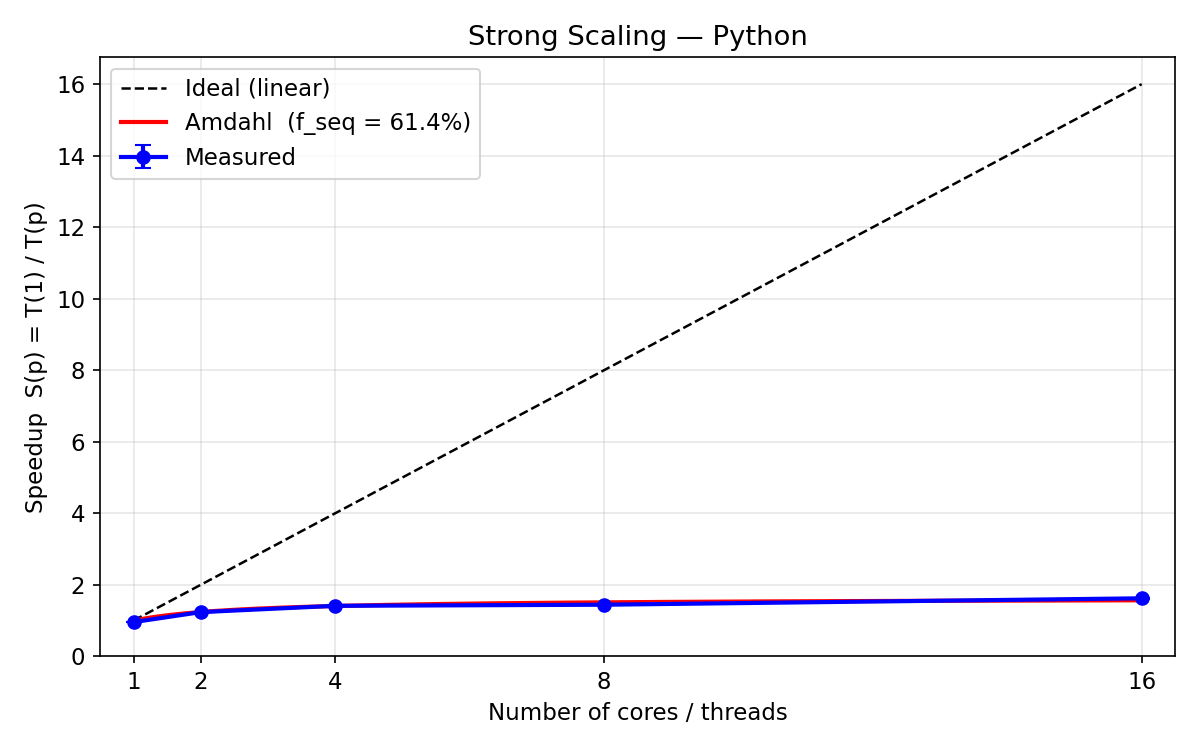
\includegraphics[width=0.82\linewidth]{benchmark/plots/strong_python.png}
    \caption{Jako skaliranje --- Python. Prikazano je izmereno ubrzanje sa granicama grešaka,
             Amdahlov fit i idealna linearna kriva.}
\end{figure}

\textbf{Analiza:} Python paralelna implementacija pokazuje slab skalabilitet. Prilagođeni
sekvencijalni udeo od 61{,}4\% je iznenađujuće visok i direktno je uzrokovan
IPC overhead-om koji nastaje razmenom ghost row-ova kroz Queue. Svaki od 500 koraka zahteva
$2P$ Queue operacija, pri čemu se svaki red pikla, šalje kroz OS pipe i depikla ---
što dodaje $\sim$70\,ms po iteraciji overhead-a bez obzira na broj jezgara.

\subsection{Rust}

Sekvencijalni referentni čas: $T_{\mathrm{seq}} = 2{,}860 \pm 0{,}039$\,s.

\begin{table}[H]
    \centering
    \caption{Jako skaliranje --- Rust}
    \begin{tabular}{rrrrrc}
        \toprule
        Jezgra & $\bar{T}$ [s] & $\sigma$ [s] & $S(p)$ & Efikasnost [\%] & Autsajderi \\
        \midrule
        1  & 2{,}841 & 0{,}062 & 1{,}007 & 100{,}6 &  0 \\
        2  & 1{,}718 & 0{,}045 & 1{,}665 &  83{,}2 &  2 \\
        4  & 1{,}320 & 0{,}005 & 2{,}166 &  54{,}1 &  1 \\
        8  & 1{,}360 & 0{,}007 & 2{,}103 &  26{,}3 &  1 \\
        16 & 1{,}895 & 0{,}009 & 1{,}509 &   9{,}4 &  0 \\
        \bottomrule
    \end{tabular}
\end{table}

\textbf{Amdahlov zakon:} Prilagođavanjem izmerenih ubrzanja:
\begin{align}
    f_{\mathrm{seq}} &= 46{,}1\% \quad \Rightarrow \quad f_{\mathrm{par}} = 53{,}9\% \\
    S_{\max} &= \frac{1}{f_{\mathrm{seq}}} = 2{,}17\times \quad (\text{beskonačno jezgara})
\end{align}

\begin{figure}[H]
    \centering
    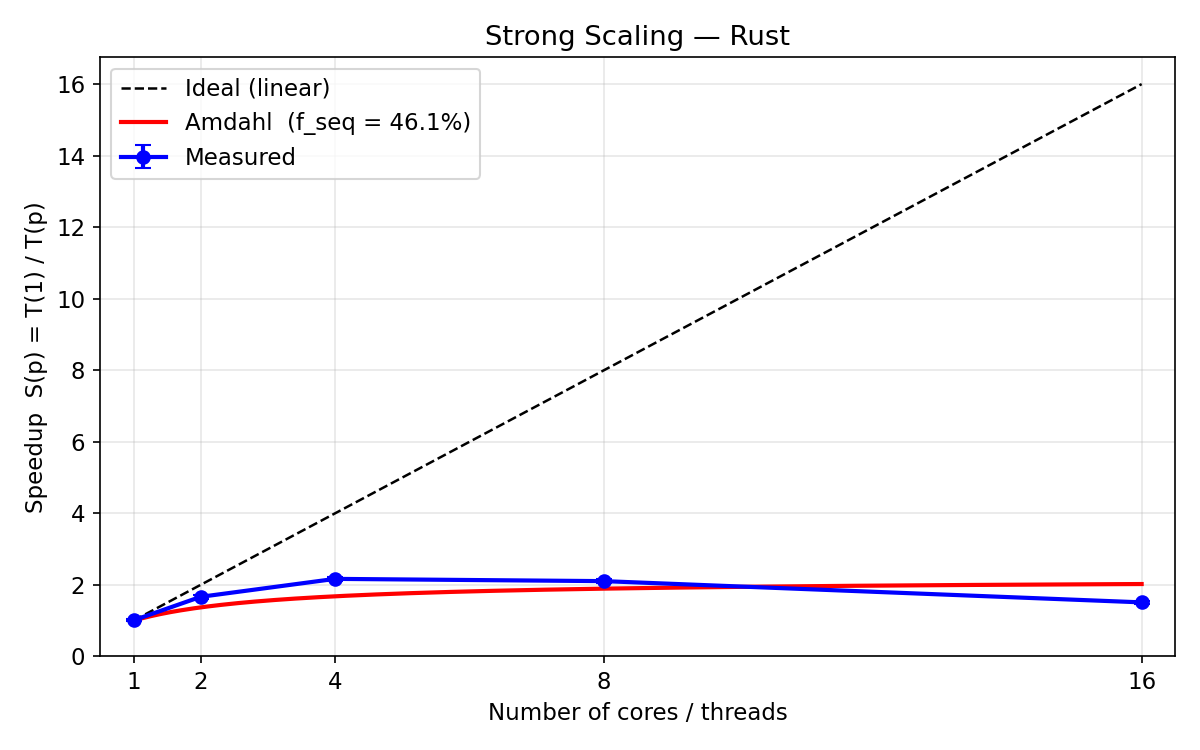
\includegraphics[width=0.82\linewidth]{benchmark/plots/strong_rust.png}
    \caption{Jako skaliranje --- Rust. Ubrzanje je nemonotonično: raste do $p=4$,
             opada za $p=8$ i $p=16$.}
\end{figure}

\textbf{Analiza:} Rust paralelna implementacija pokazuje neočekivano nemonotonično ubrzanje.
Optimum je pri $p=4$ (4 fizička jezgra), dok se ubrzanje smanjuje za $p=8$ i $p=16$.
Ovo se objašnjava:
\begin{itemize}[noitemsep]
    \item \textbf{$p=4$ (fizička jezgra):} AVX2 vektorizacija je aktivna, sva fizička jezgra
          rade nezavisno, ubrzanje $= 2{,}17\times$.
    \item \textbf{$p=8$ (Hyper-Threading):} Simulacija je \emph{memory-bandwidth-bound} ---
          HT jezgra dele iste pipelines za čitanje/pisanje i ne doprinose dodatnom ubrzanju.
    \item \textbf{$p=16$ (Rayon overhead):} Rayon mora da raspodeli 5000 redova na 16 threadova
          uz task dispatch overhead koji premašuje dobit, a 16 threadova deli isti L3 cache.
\end{itemize}

Amdahlov zakon daje loš fit za nemonotonične podatke: kriva kompromisuje tako što je
iznad merenih vrednosti za malo $p$ i ispod za $p=16$. Realni $f_{\mathrm{seq}}$ je niži
od izmerenog 46{,}1\% --- \emph{stvarno} ograničenje je propusnost memorijske magistrale,
ne sekvencijalni kod.

%  rezultati --- slabo skaliranje
\section{Rezultati --- Slabo skaliranje}

\subsection{Python}

Bazno vreme (p=1, mreža $2500\!\times\!2500$, 200 iteracija): $T(1) = 7{,}134 \pm 0{,}243$\,s.

\begin{table}[H]
    \centering
    \caption{Slabo skaliranje --- Python}
    \begin{tabular}{rrlrrrc}
        \toprule
        $p$ & Mreža & $\bar{T}$ [s] & $\sigma$ [s] & $S_{\mathrm{sc}}(p)$ & Efikasnost [\%] & Autsajderi \\
        \midrule
        1  & $2500\!\times\!2500$   &  7{,}134 & 0{,}243 & 1{,}000 & 100{,}0 & 1 \\
        2  & $3536\!\times\!3536$   & 10{,}176 & 0{,}188 & 1{,}402 &  70{,}1 & 4 \\
        4  & $5000\!\times\!5000$   & 16{,}293 & 0{,}034 & 1{,}751 &  43{,}8 & 2 \\
        8  & $7071\!\times\!7071$   & 30{,}430 & 0{,}210 & 1{,}875 &  23{,}4 & 0 \\
        16 & $10000\!\times\!10000$ & 54{,}230 & 0{,}124 & 2{,}105 &  13{,}2 & 2 \\
        \bottomrule
    \end{tabular}
\end{table}

\textbf{Gustafsonov zakon:} Prilagođavanjem izmerenih skaliranih ubrzanja:
\begin{equation}
    f_{\mathrm{seq}} = 91{,}1\% \quad \Rightarrow \quad f_{\mathrm{par}} = 8{,}9\%
\end{equation}

\begin{figure}[H]
    \centering
    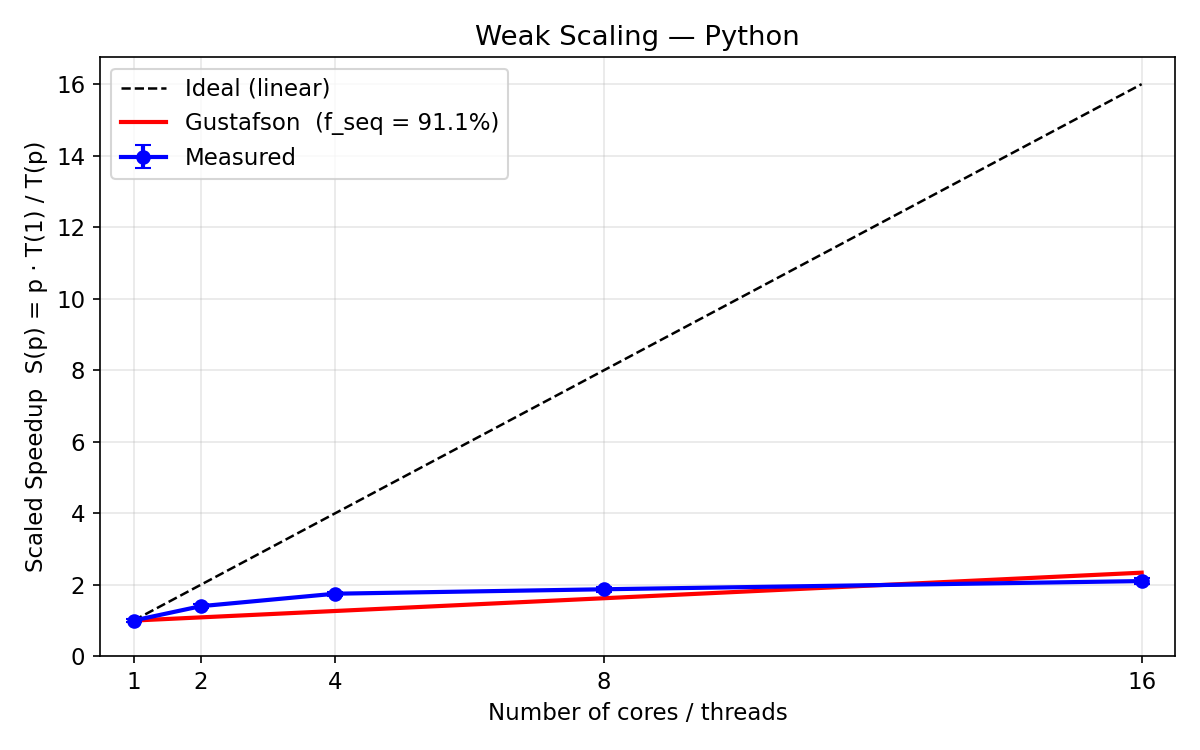
\includegraphics[width=0.82\linewidth]{benchmark/plots/weak_python.png}
    \caption{Slabo skaliranje --- Python. Skalirani napon raste sa $p$ ali daleko ispod ideala.}
\end{figure}

\textbf{Analiza:} Gustafsonov sekvencijalni udeo od 91{,}1\% potvrđuje dominantnost IPC overhead-a.
Dok se broj ćelija po procesu ne menja, Queue overhead \emph{raste} sa mreže jer
$\lfloor 2500\sqrt{p} \rfloor$ redova je dužine $N \propto \sqrt{p}$, pa se i ghost row-ovi
povećavaju sa $p$. Serializacija i prenos većih nizova dominiše ukupnim vremenom.

\subsection{Rust}

Bazno vreme (p=1, mreža $2500\!\times\!2500$, 200 iteracija): $T(1) = 0{,}361 \pm 0{,}027$\,s.

\begin{table}[H]
    \centering
    \caption{Slabo skaliranje --- Rust}
    \begin{tabular}{rrlrrrc}
        \toprule
        $p$ & Mreža & $\bar{T}$ [s] & $\sigma$ [s] & $S_{\mathrm{sc}}(p)$ & Efikasnost [\%] & Autsajderi \\
        \midrule
        1  & $2500\!\times\!2500$   & 0{,}361 & 0{,}027 & 1{,}000 & 100{,}0 & 3 \\
        2  & $3536\!\times\!3536$   & 0{,}406 & 0{,}010 & 1{,}777 &  88{,}8 & 3 \\
        4  & $5000\!\times\!5000$   & 0{,}537 & 0{,}002 & 2{,}690 &  67{,}2 & 1 \\
        8  & $7071\!\times\!7071$   & 1{,}116 & 0{,}002 & 2{,}586 &  32{,}3 & 2 \\
        16 & $10000\!\times\!10000$ & 2{,}465 & 0{,}007 & 2{,}342 &  14{,}6 & 1 \\
        \bottomrule
    \end{tabular}
\end{table}

\textbf{Gustafsonov zakon:} Prilagođavanjem izmerenih skaliranih ubrzanja:
\begin{equation}
    f_{\mathrm{seq}} = 87{,}0\% \quad \Rightarrow \quad f_{\mathrm{par}} = 13{,}0\%
\end{equation}

\begin{figure}[H]
    \centering
    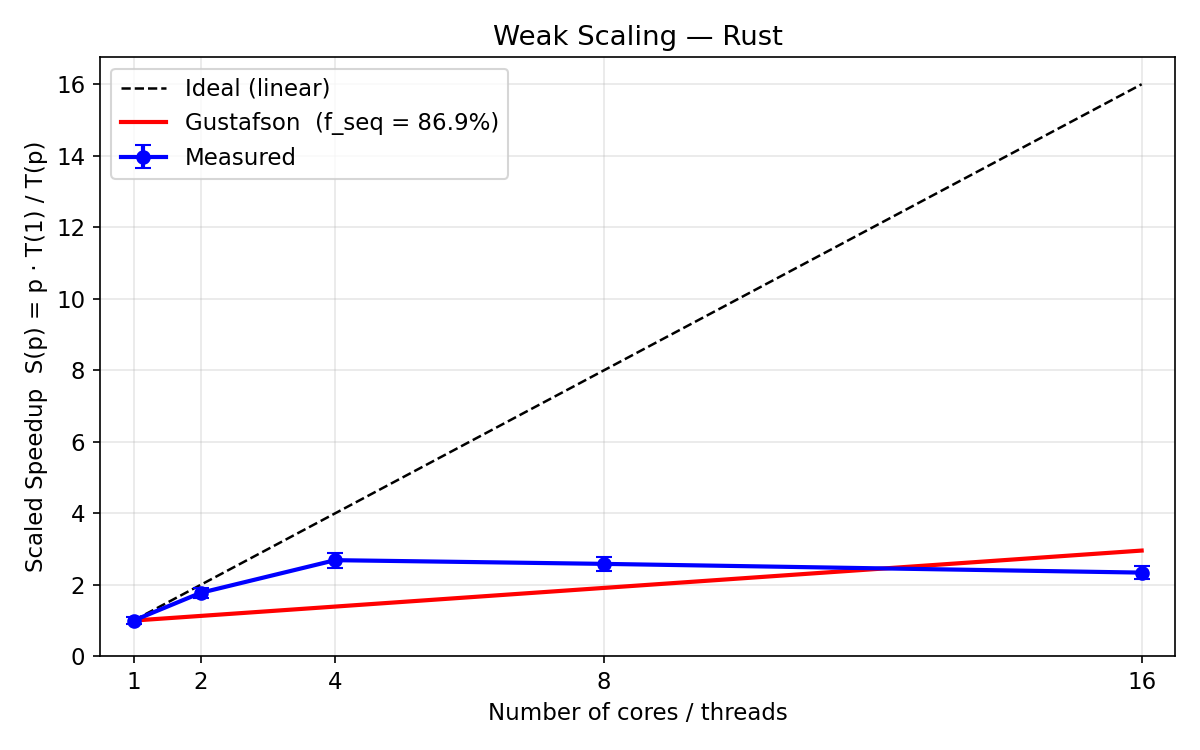
\includegraphics[width=0.82\linewidth]{benchmark/plots/weak_rust.png}
    \caption{Slabo skaliranje --- Rust. Skalirani napon dostiže maksimum pri $p=4$ (fizička jezgra),
             a zatim opada zbog bandwidth saturacije.}
\end{figure}

\textbf{Analiza:} Rust slabo skaliranje pokazuje isti nemonotonični obrazac kao jako skaliranje.
$S_{\mathrm{sc}}$ dostiže maksimum pri $p=4$ ($S_{\mathrm{sc}} = 2{,}69$) i zatim opada za
$p=8$ i $p=16$ iz istog razloga: veće mreže traže više memorijskog propusnog opsega i sistem
dostiže bandwidth limit na 4 fizička jezgra.

%  analiza i zaključci
\section{Analiza i zaključci}

\subsection{Sekvencijalni nasuprot paralelnog dela koda}

\begin{table}[H]
    \centering
    \caption{Procenjeni sekvencijalni i paralelni udeli koda}
    \begin{tabular}{llll}
        \toprule
        \textbf{Implementacija} & $f_{\mathrm{seq}}$ & $f_{\mathrm{par}}$ & \textbf{Dominantno ograničenje} \\
        \midrule
        Python (jako sk.) & 61{,}4\% & 38{,}6\% & IPC Queue overhead \\
        Rust (jako sk.)   & 46{,}1\% & 53{,}9\% & Memorijska magistrala \\
        Python (slabo sk.)& 91{,}1\% &  8{,}9\% & IPC Queue overhead + rast ghost row-ova \\
        Rust (slabo sk.)  & 87{,}0\% & 13{,}0\% & Memorijska magistrala \\
        \bottomrule
    \end{tabular}
\end{table}

\textbf{Python:} Sekvencijalni deo (inicijalizacija mreže, skupljanje rezultata, serializacija
ghost row-ova kroz Queue) dominira ukupnim vremenom. IPC mehanizam uvodi $O(N)$ overhead
po iteraciji koji je neelastičan u odnosu na broj jezgara.

\textbf{Rust:} Sekvencijalni deo (inicijalizacija mreže, Rayon task dispatch) je zanemarljiv.
Prividno visoki $f_{\mathrm{seq}}$ iz Amdahlove analize je artefakt nemonootoničnog profila
ubrzanja --- stvarno ograničenje je propusnost memorijske magistrale DDR4-2400 ($\approx$38\,GB/s)
koja se saturiše pri 4 fizička jezgra.

\subsection{Poređenje Python nasuprot Rust}

\begin{table}[H]
    \centering
    \caption{Poređenje implementacija --- jako skaliranje ($5000\times5000$, 500 iter.)}
    \begin{tabular}{lrrr}
        \toprule
        \textbf{Implementacija} & \textbf{Seq} & \textbf{Par ($p=4$)} & \textbf{Par ($p=8$)} \\
        \midrule
        Python & 56{,}957\,s & 40{,}322\,s & 39{,}468\,s \\
        Rust   & 2{,}860\,s  & 1{,}320\,s  & 1{,}360\,s  \\
        \midrule
        Rust / Python ubrzanje & $\mathbf{19{,}9\times}$ & $\mathbf{30{,}5\times}$ & $\mathbf{29{,}0\times}$ \\
        \bottomrule
    \end{tabular}
\end{table}

Rust je dramatično brži od Pythona zahvaljujući:
\begin{enumerate}[noitemsep]
    \item \textbf{AVX2 auto-vektorizaciji:} Unutrašnja petlja obrađuje 32 ćelije po SIMD ciklusu
          umesto jedne ćelije po NumPy operaciji.
    \item \textbf{Nultom IPC overhead:} Rayon threadovi dele memoriju direktno --- nema serializacije,
          pikla ni OS pipe-ova.
    \item \textbf{Branchless pravilima:} Eliminacija conditionalnih grananja omogućava SIMD izvršavanje
          bez prediktivnog kašnjenja.
    \item \textbf{Eliminacija bounds check:} Row-slice pristup uklanja provere granica za unutrašnje
          kolone, što smanjuje broj instrukcija po ćeliji.
\end{enumerate}

Python je ograničen IPC overhead-om kroz Queue koji dominira i čini dalji porast $p$
praktično beznačajnim.

\subsection{Zaključak}

Projekat demonstrira ključne razlike u paralelizacionim strategijama:

\begin{itemize}
    \item \textbf{Python + multiprocessing:} Pogodan za implementaciju ali teško skalabilan
          zbog IPC overhead-a. Optimalna vrednost $p$ je 16 (samo 43\% poboljšanje u odnosu na
          sekvencijalnu verziju), a dalji rast $p$ donosi minimalne koristi.

    \item \textbf{Rust + Rayon:} Efikasan do limita memorijske magistrale. Optimalna vrednost $p$
          je 4 (broj fizičkih jezgara, 2{,}17$\times$ ubrzanje), a Hyper-Threading ne donosi
          dodatne koristi jer je problem \emph{bandwidth-bound}.

    \item \textbf{Amdahlov zakon} dobro opisuje monotonično skaliranje (Python), ali daje
          loš fit za sisteme koji dostižu hardverske limite pre dobitaka od paralelizacije (Rust).

    \item \textbf{Gustafsonov zakon} potvrđuje da čak i pri rastu posla, Python ne može
          da iskoristi dodatna jezgra zbog dominantnog overhead-a, dok Rust postiže dobro
          skaliranje do 4 fizička jezgra.
\end{itemize}

Ukupni zaključak: za numerički intenzivne aplikacije kao što je simulacija celularnog automata,
Rust sa SIMD optimizacijom i shared-memory paralelizmom nudi dramatično superiorne performanse
u poređenju sa Python multiprocessing pristupom, posebno na sistemima sa ograničenim brojem
memorijskih kanala.

\end{document}
